\chapter{\LaTeX の書き方}
\label{chap:latex}

この章では,よく使う\LaTeX のコマンドを説明する.足りない部分はぐぐればだいたいわかると思う.最初に書いておくと,数式を書く方法は,ぼく自身使わなかったので書いていない.ぼくのいた研究室でごりごり数式をたくさん書く必要のあるひとは,研究の種類からするとあまり居ない気がする.

\section{主なコマンド}

\subsection{章と節}

文書構造を明確にする大事なもの.目次はこれらのコマンドをもとに作られる.例えば,この第\ref{chap:latex}章の冒頭部分はこのようなソースで書かれている.

\begin{itembox}[l]{\texttt{03.tex}}
\begin{verbatim}
\chapter{\LaTeX の書き方}
\label{chap:latex}

この章では,よく使う\LaTeX のコマンドを説明する.(略)

\section{主なコマンド}

\subsection{章と節}

文書構造を明確にする大事なもの.目次はこれらのコマンドをもとに作られる.例えば,この第\ref{chap:latex}章の冒頭部分はこのようなソースで書かれている.
\end{verbatim}
\end{itembox}

章は \verb|\chapter{見出し}|,節は \verb|\section{見出し}|,小節は \verb|\subsection{見出し}|,小々節は \verb|\subsubsection{見出し}| を使う.表\ref{tb:chap}に一覧する.

\begin{table}[htbp]
  \caption{章と節のコマンド}
  \label{tb:chap}
  \begin{center}
    \begin{tabular}{@{}cc@{}}
      \toprule
      コマンド & 用途 \\ \midrule
      \verb|\chapter{見出し}| & 章 \\
      \verb|\section{見出し}| & 節 \\
      \verb|\subsection{見出し}| & 小節 \\
      \verb|\subsubsection{見出し}| & 小々節 \\ \bottomrule
    \end{tabular}
  \end{center}
\end{table}

\subsubsection{小々節見出しサンプルその1}

小々節は上のように \verb|\subsubsection{タイトル}| で書けるけれど,あまり文書の階層構造が深いことは望ましくないので,多用しなければならないようなら文書構造を見直したほうがよいと思う.

\subsubsection{小々節見出しサンプルその2}

小々節は,章や節,小節のように \texttt{N.N.N} といった番号ではなくて,括弧付きの番号で出力される.かつ,目次には出力されない.

\subsection{図}

図は次のように出力される(図\ref{fig:sample1}).

\begin{figure}[htbp]
    \begin{center}
       \fbox{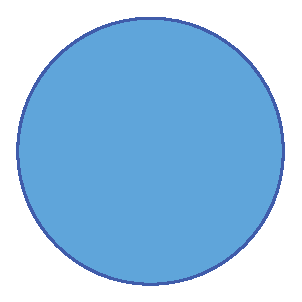
\includegraphics[width=50mm]{./image/image.eps}}
    \end{center}
    \caption{図の例}
    \label{fig:sample1}
\end{figure}

ソースでは次のように記述している.

\begin{itembox}[l]{\texttt{03.tex}}
\begin{verbatim}
図は次のように出力される(図\ref{fig:sample1}).

\begin{figure}[htbp]
    \begin{center}
       \fbox{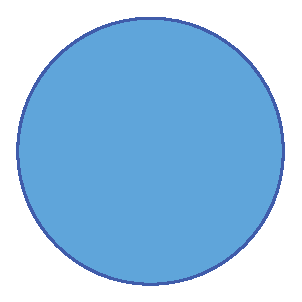
\includegraphics[width=40mm]{./image/image.eps}}
    \end{center}
    \caption{図の例}
    \label{fig:sample1}
\end{figure}
\end{verbatim}
\end{itembox}

\verb|\begin{figure}[htbp]|  の\texttt{htbp}は,表示位置の優先順位の設定.基本的に\LaTeX では,図の挿入位置は強制的には指定できない.いくつか候補を指定しておくと,候補のなかの優先度の高い順に,図を入れられるスペースがあるかどうかを調べて,入れられればそこに,入れられなければ次の候補のスペースを調べる,という処理が行われる.\texttt{h}はこのコマンドを書いたその場所に,\texttt{t}はページの一番上に,\texttt{b}はページの一番下に,\texttt{p}は画像だけ別ページに,それぞれ配置する.基本的には\texttt{htbp}のように全部書いておけば問題ない.

\verb|\includegraphics| コマンドで,図のサイズと挿入するファイルを指定する.上の例ではサイズは \texttt{width=50mm} として幅を指定したけれど,ここは他にも \texttt{height=30mm} として高さを指定してもよいし,\texttt{scale=0.5} として拡大率を指定してもよい.画像は最近の \LaTeX 環境であれば\texttt{*.eps}以外でも使える.ただし,\texttt{bb} (Bounding Box) として画像の大きさを指定する必要があることも多い.
以下はJPEG画像を使用する例.

\begin{itembox}[l]{\texttt{03.tex}}
\begin{verbatim}
\begin{figure}[htbp]
    \begin{center}
       \fbox{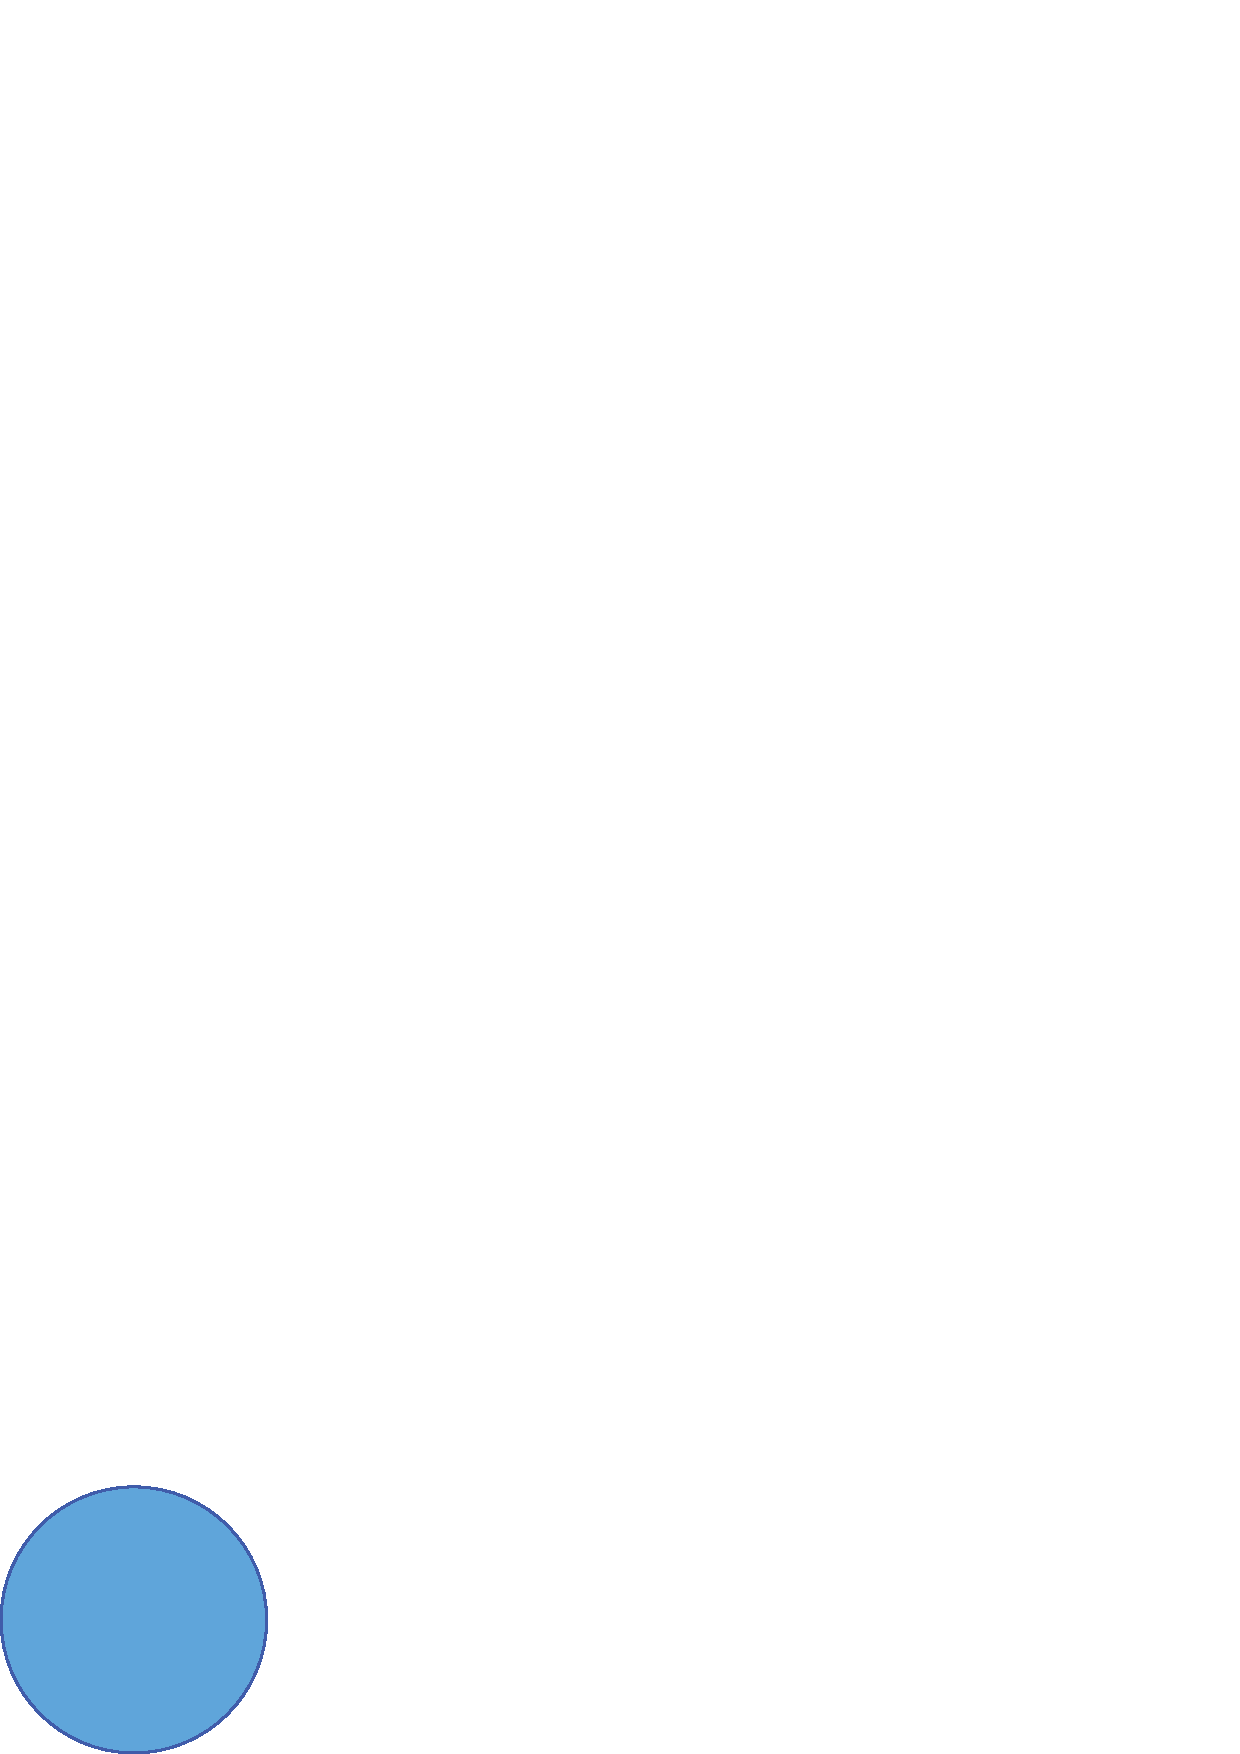
\includegraphics[width=40mm,bb=0 0 640 480]{image.jpg}}
    \end{center}
    \caption{図の例}
    \label{fig:sample1}
\end{figure}
\end{verbatim}
\end{itembox}

bbの指定は,上記のように\texttt{*.tex} ファイルの中で指定してもいいが,
\texttt{*.bb}ファイルを作っておく方法もある.
ターミナルで\texttt{ebb}コマンドを使用すると\texttt{*.bb}ファイルを簡単に作れる.


\begin{itembox}[l]{ebbコマンドの例}
\begin{verbatim}
% ebb image.jpg
\end{verbatim}
\end{itembox}


\verb|\includegraphics| を \verb|\fbox| に入れると,画像に枠を付けられる.

\verb|\caption| コマンドで図の見出しを指定できる.図の見出しは,図の下に表記するので注意.ここで指定した見出しが,図の目次に表示される.

\verb|\label| コマンドでは図の参照用ラベルを設定できる.本文中,\verb|\ref| コマンドで参照用ラベルを指定すると,対応した図の番号が自動的に挿入される.これも目次や参考文献と同様,最低二回のコンパイルが必要なので注意.

図を二つ横に並べたい場合は,次のように書く(図\ref{fig:sample2},図\ref{fig:sample3}).

\begin{figure}[htbp]
  \begin{minipage}{0.5\hsize}
    \begin{center}
       \fbox{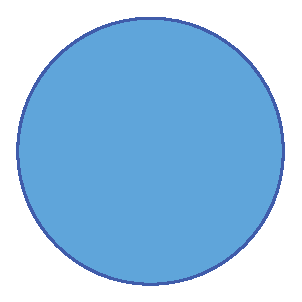
\includegraphics[width=40mm]{./image/image.eps}}
    \end{center}
    \caption{図を並べる例1}
    \label{fig:sample2}
  \end{minipage}
  \begin{minipage}{0.5\hsize}
    \begin{center}
       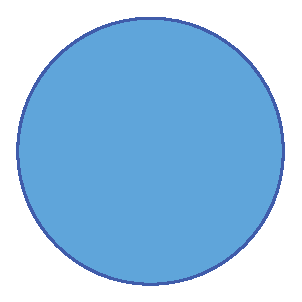
\includegraphics[width=40mm]{./image/image.eps}
    \end{center}
    \caption{図を並べる例2,枠なし}
    \label{fig:sample3}
  \end{minipage}
\end{figure}

\begin{itembox}[l]{\texttt{03.tex}}
\begin{verbatim}
図を二つ横に並べたい場合は,次のように書く(図\ref{fig:sample2},図\ref{fig:sample3}).

\begin{figure}[htbp]
  \begin{minipage}{0.5\hsize}
    \begin{center}
       \fbox{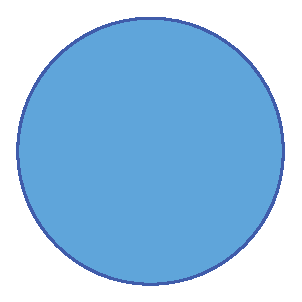
\includegraphics[width=40mm]{./image/image.eps}}
    \end{center}
    \caption{図を並べる例1}
    \label{fig:sample2}
  \end{minipage}
  \begin{minipage}{0.5\hsize}
    \begin{center}
       \fbox{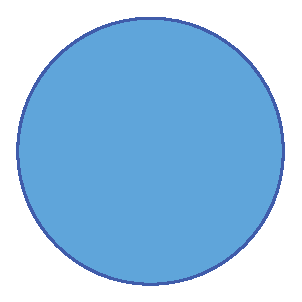
\includegraphics[width=40mm]{./image/image.eps}}
    \end{center}
    \caption{図を並べる例2}
    \label{fig:sample3}
  \end{minipage}
\end{figure}
\end{verbatim}
\end{itembox}


\subsection{表}

表は次のように出力される(表\ref{tb:sample1}).

\begin{table}[htbp]
  \caption{表の例}
  \label{tb:sample1}
  \begin{center}
    \begin{tabular}{@{}lcc@{}}
      \toprule
      種類 & 味 & 評価 \\ \midrule
      ドラ焼き & 甘い & 好き \\
      メロンパン & カリもふ & 好き \\
      クリームパン & 神 & すごく好き \\ \bottomrule
      \end{tabular}
  \end{center}
\end{table}

ソースでは次のようになっている.

\begin{itembox}[l]{\texttt{03.tex}}
\begin{verbatim}
表は次のように出力される(表\ref{tb:sample1}).

\begin{table}[htbp]
  \caption{表の例}
  \label{tb:sample1}
  \begin{center}
    \begin{tabular}{@{}lcc@{}}
      \toprule
      種類 & 味 & 評価 \\ \midrule
      ドラ焼き & 甘い & 好き \\
      メロンパン & カリもふ & 好き \\
      クリームパン & 神 & すごく好き \\ \bottomrule
      \end{tabular}
  \end{center}
\end{table}
\end{verbatim}
\end{itembox}

\texttt{htbp}や \verb|\caption| と \verb|\label| は図と同様.ただし表のタイトルは表の上に書く.

セルの中の文字は,\texttt{\&}で区切って並べる.行と行は \verb|\\| で区切る.水平方向の罫線が必要なら,\verb|\hline| を書く.

水平方向や垂直方向のセルの結合もできる.例を示すので,くわしくはぐぐろう.説明がめんどう.\verb|\multirow|,\verb|\multicolumn|,\verb|\cline| を使うとできる.

\begin{table}[htbp]
  \caption{セルを結合した例}
  \label{tb:sample2}
  \begin{center}
  \begin{tabular}{c|c|c}
    \hline
    ほげ&ふー&ばー\\\hline\hline
    \multirow{2}{*}{ほげほげ}&\multicolumn{2}{c}{ふーふー} \\\cline{2-3}
    &ふーふーふー&ばーばーばー\\\hline
  \end{tabular}
  \end{center}
\end{table}

\begin{itembox}[l]{\texttt{03.tex}}
\begin{verbatim}
\begin{table}[htbp]
  \caption{セルを結合した例}
  \label{tb:sample2}
  \begin{center}
  \begin{tabular}{c|c|c}
    \hline
    ほげ&ふー&ばー\\\hline\hline
    \multirow{2}{*}{ほげほげ}&\multicolumn{2}{c}{ふーふー} \\\cline{2-3}
    &ふーふーふー&ばーばーばー\\\hline
  \end{tabular}
  \end{center}
\end{table}
\end{verbatim}
\end{itembox}


\subsection{脚注}

脚注は \verb|\footnote| コマンドを使う.例えばこんな感じ\footnote{ページの下に小さく説明を出せる}.

\begin{itembox}[l]{\texttt{03.tex}}
\begin{verbatim}
例えばこんな感じ\footnote{ページの下に小さく説明を出せる}.
\end{verbatim}
\end{itembox}

\section{その他のコマンド}

ぐぐる\footnote{http://www.google.co.jp/}.

特殊なことは何もしていないテンプレートなので,ぐぐって出たことはだいたいそのまま何でも使える.

あるいは,このファイル自体も\LaTeX で書かれているわけだから,これの\texttt{*.tex}を見るのもよいかもしれない.
